\documentclass[xcolor={dvipsnames,table}]{beamer}

\usepackage[utf8]{inputenc}
\usepackage[brazil]{babel}
\usepackage{amsmath, amssymb}
\usepackage{physics}
\usepackage{color}
% \usepackage[table]{xcolor}

\usetheme{Madrid}


% ---------------------
% Pacotes Tikzi
% ---------------------
\usepackage{tikz}
\usetikzlibrary{arrows.meta}



\title[Abordagem de Computação Quântica para Problemas de Otimização]{Uma Abordagem de Computação Quântica de Variáveis Contínuas para Otimização Combinatória: Aplicações ao Problema de Roteamento de Veículos}
\author[Clovis Caface]{Clovis Aparecido Caface Filho \\[1ex]
\textbf{Orientação}: Prof. Dr. Raphael Yokoingawa de Camargo \\
\textbf{Coorientação}: Dr. Tiago de Souza Farias}
\institute{UFABC}
\date{2026}

\begin{document}

\frame{\titlepage}

\frame{ 
    \tableofcontents
}

%------------------------------------------------
\section{Fundamentação}
\subsection{Problemas de Rotas de Veículos}

\begin{frame}{Problemas de Rotas de Veículos - VRP}
    \begin{itemize}
        \item Minimizar o custo das rotas de uma frota de veículos no atendimento a clientes
        \item Ampla variedade de aplicações
        \begin{itemize}
            \item coleta de resíduos
            \item distribuição de mercadorias
            \item transporte escolar 
            \item rotas de serviços emergenciais 
        \end{itemize}
        \item NP-Difícil
    \end{itemize}
\end{frame}

\begin{frame}{VRP}
    \begin{center}
        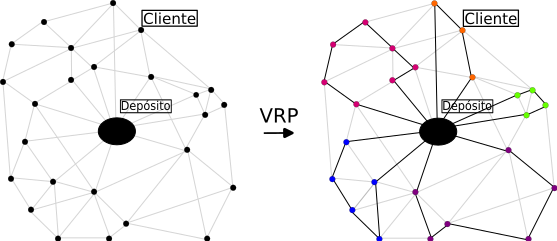
\includegraphics[width=0.75\textwidth,keepaspectratio]{figs/vrp.png}
    \end{center}
    \vfill
    \begin{minipage}[c]{\textwidth}
        \centering
        \tiny{\textbf{Fonte}: Autoria própria (2026)}
    \end{minipage}
\end{frame}

\begin{frame}{VRP - caso particular TSP}
    \begin{center}
        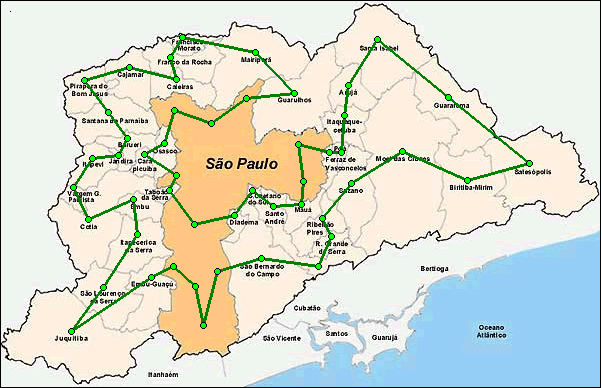
\includegraphics[width=.65\textwidth]{figs/tsp.png}
    \end{center}
    \vfill
    \begin{minipage}[c]{\textwidth}
        \centering
        \tiny{\textbf{Fonte}: Autoria própria (2026)}
    \end{minipage}
\end{frame}

\begin{frame}{VRP}
    \begin{block}{Modelagem Matemática}
        Decisão Binária
        $$
            x_{ijk}=\begin{cases}
                1, \text{se o veículo } k \text{ percorre o arco } (i,j) \\
                0, \text{caso contrário}
            \end{cases}
        $$
            A função objetivo consiste em minimizar o custo total das rotas % sujeita às restrições do problema
            $$
                \min \sum_{k\in K}^{max}\sum_{i \in V} \sum_{\substack{j \in V \\ j \neq i}} c_{ijk}\, x_{ijk}
            $$
    \end{block}
\end{frame}


\begin{frame}{VRP}
    \begin{minipage}[c]{0.45\textwidth}
        \begin{block}{Restrições}
            Sujeito a restrição de visita 
            $$
            \sum_{k\in K}\sum_{\substack{j \in V \\ j \neq i}}x_{ijk}=1,\forall j\in V\setminus\{0\}
            $$
            $$
            \sum_{k\in K}\sum_{\substack{i \in V \\ i \neq j}}x_{ijk}=1,\forall i\in V\setminus\{0\}
            $$
        \end{block}
    \end{minipage}
    \hfill
    \begin{minipage}[c]{0.45\textwidth}
        \begin{block}{Restrições}
            Sujeito também a restrição de fluxo do depósito
            $$
                \sum_{k\in K}\sum_{\substack{j \in V \\ j \neq i}}x_{i0k}=1,\forall i\in V\setminus\{0\}
            $$
            $$
                \sum_{k\in K}\sum_{\substack{i \in V \\ i \neq j}}x_{0jk}=1,\forall i\in V\setminus\{0\}
            $$
        \end{block}
    \end{minipage}
\end{frame}

\begin{frame}{VRP}
    \begin{block}{Função Custo}
        \begin{equation*}
            \begin{aligned}
                C(\mathbf{x})= & \sum_{k\in K}\sum_{i \in V} \sum_{\substack{j \in V \\ j \neq i}} c_{ijk}\, x_{ijk}  \\
                & + \alpha\left(\sum_{k\in K}\sum_{\substack{j \in V \\ j \neq i}}x_{ijk}-1\right)^2 + \beta\left( \sum_{k\in K}\sum_{\substack{i \in V \\ i \neq j}}x_{ijk}-1\right)^2 \\
                & + \gamma\left(\sum_{k\in K}\sum_{\substack{j \in V \\ j \neq i}}x_{0jk}-1\right)^2 + \lambda\left( \sum_{k\in K}\sum_{\substack{i \in V \\ i \neq j}}x_{i0k}-1\right)^2
            \end{aligned}
        \end{equation*}
        onde $\alpha, \beta, \gamma$ e $\lambda$ são hiperparâmetros do modelo.
    \end{block}
    
\end{frame}


\begin{frame}{VRP}
    \begin{block}{Diversas Variantes}
        \begin{itemize}
            \item Capacitado:\quad $\sum_{i\in V}\sum_{\substack{j\in V\\j\neq i}}d_jx_{ijk}\leq Q,\ \forall k\in K$
            \item Janela de tempo:\quad $a_i\leq T_i\leq b_i,\ \forall i\in V$
            \item Multiplos depósitos
            \item Taxi 
        \end{itemize}
    \end{block}
\end{frame}

%------------------------------------------------
\subsection{Abordagem Clássica}
\begin{frame}{Abordagem Clássica}
    \begin{itemize}
        \item Força Bruta
        \item Heurísticas Meta-heuristicas
        \begin{itemize}
            \item Guloso
            \item Tabu
            \item Algoritmo Genético    
            \item Colônia de Formigas
        \end{itemize}
    \end{itemize}
\end{frame}

%------------------------------------------------
\subsection{Computação Quântica de Variáveis Contínuas}
\begin{frame}{Computação Quântica}
    
    \begin{minipage}[c]{0.45\textwidth}
        \centering
        % \caption{Esfera de Bloch para $\ket{\psi}$}    
        \begin{tikzpicture}[line cap=round, line join=round, >=Triangle]
            \clip(-2.19,-2.49) rectangle (2.66,2.58);
            \draw [shift={(0,0)}, lightgray, fill, fill opacity=0.1] (0,0) -- (56.7:0.4) arc (56.7:90.:0.4) -- cycle;
            \draw [shift={(0,0)}, lightgray, fill, fill opacity=0.1] (0,0) -- (-135.7:0.4) arc (-135.7:-33.2:0.4) -- cycle;
            \draw(0,0) circle (2cm);
            \draw [rotate around={0.:(0.,0.)},dash pattern=on 3pt off 3pt] (0,0) ellipse (2cm and 0.9cm);
            \draw (0,0)-- (0.70,1.07);
            \draw [->] (0,0) -- (0,2);
            \draw [->] (0,0) -- (-0.81,-0.79);
            \draw [->] (0,0) -- (2,0);
            \draw [dotted] (0.7,1)-- (0.7,-0.46);
            \draw [dotted] (0,0)-- (0.7,-0.46);
            \draw (-0.08,-0.3) node[anchor=north west] {$\varphi$};
            \draw (0.01,0.9) node[anchor=north west] {$\theta$};
            \draw (-1.01,-0.72) node[anchor=north west] {$x$};
            \draw (2.07,0.3) node[anchor=north west] {$y$};
            \draw (-0.5,2.6) node[anchor=north west] {$\ket{0}$};
            \draw (-0.4,-2) node[anchor=north west] {$\ket{1}$};
            \draw (0.4,1.65) node[anchor=north west] {$\ket{\psi}$};
            \scriptsize
            \draw [fill] (0,0) circle (1.5pt);
            \draw [fill] (0.7,1.1) circle (0.5pt);
        \end{tikzpicture}
    \end{minipage}
    \hfill
    \begin{minipage}[c]{0.45\textwidth}
        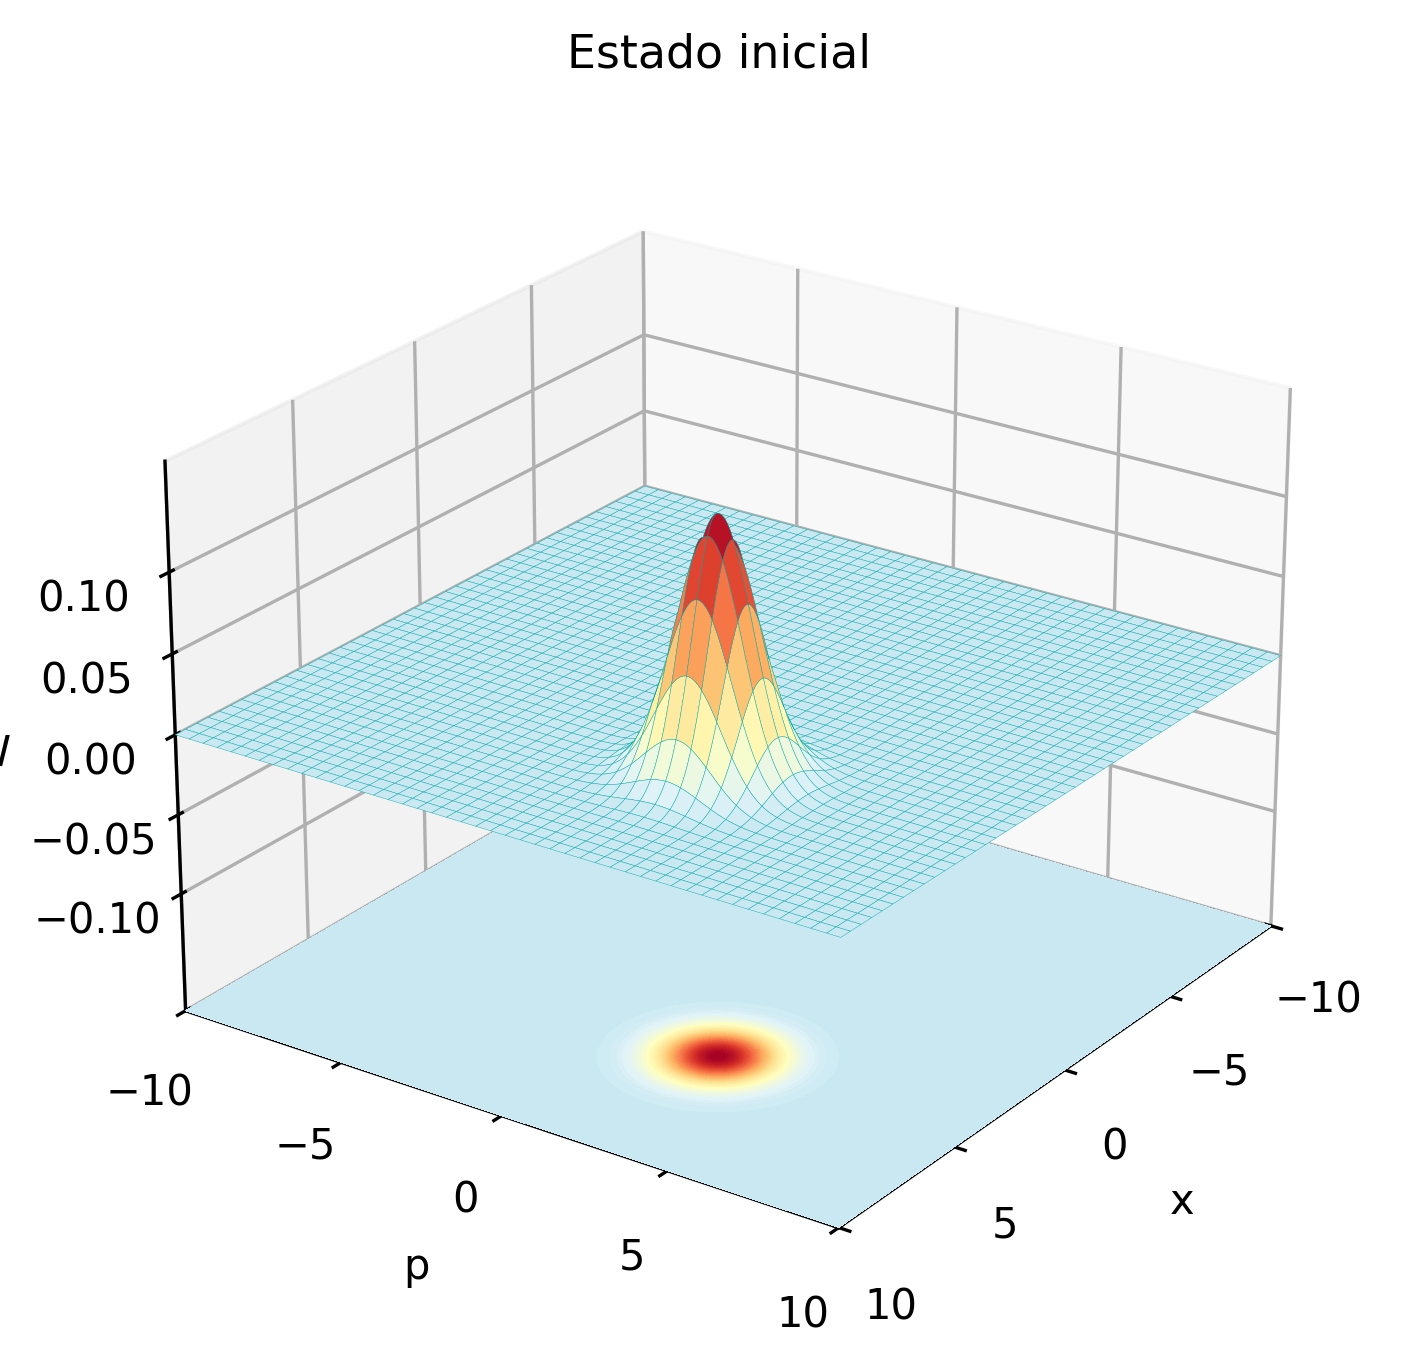
\includegraphics[width=\textwidth]{figs/coherente_state.png}
    \end{minipage}
    \vfill
    \begin{minipage}[c]{\textwidth}
        \centering
        \tiny{\textbf{Fonte}: Autoria própria (2026)}
    \end{minipage}
\end{frame}

\begin{frame}{Computação Quântica de Variáveis Contínuas}
    
    \begin{itemize}
        \item Princípio de Exclusão de Pauli $\rightarrow$ Dimensão finita (\textit{qubits, qutrits, qudits})
        \item Dimensão infinita $\rightarrow$ \textit{qumodes} (base de Fock)
        \begin{itemize}
            \item Fótons - exemplo mais proeminente
            \item Formado pelos autoestados ortonormais do operador número $$\hat{n}=\hat{a}^\dagger \hat{a}$$
            \item O estado do sistema é descrito no espaço de fase por dois observáveis
            \begin{itemize}
                \item posição: $\hat{x}=\displaystyle\frac{(\hat{a}^\dagger+\hat{a})}{\sqrt{2}}$  (amplitude do campo)
                \item momento: $\hat{p}=\displaystyle\frac{i(\hat{a}^\dagger-\hat{a})}{\sqrt{2}}$  (fase do campo)
            \end{itemize}
        \end{itemize}
    \end{itemize}
\end{frame}

\begin{frame}{Computação Quântica de Variáveis Contínuas}

    \begin{block}{Distinção Fundamental}
        \begin{itemize}
            \item Qubit $\rightarrow$ superposição de dois estados
            $$\ket{\Psi}=a\ket{0}+b\ket{1}$$
            \item Qumodes $\rightarrow$ superposição contínua
            $$\ket{\Psi}=\int\psi(x)\ket{x}\text{d}x$$
        \end{itemize}
    \end{block}
\end{frame}

\begin{frame}{Computação Quântica de Variáveis Contínuas}

    \begin{block}{Portas Gaussianas}
        
        \begin{minipage}[c]{\textwidth}
            \begin{minipage}[c]{0.45\textwidth}
                \centering
                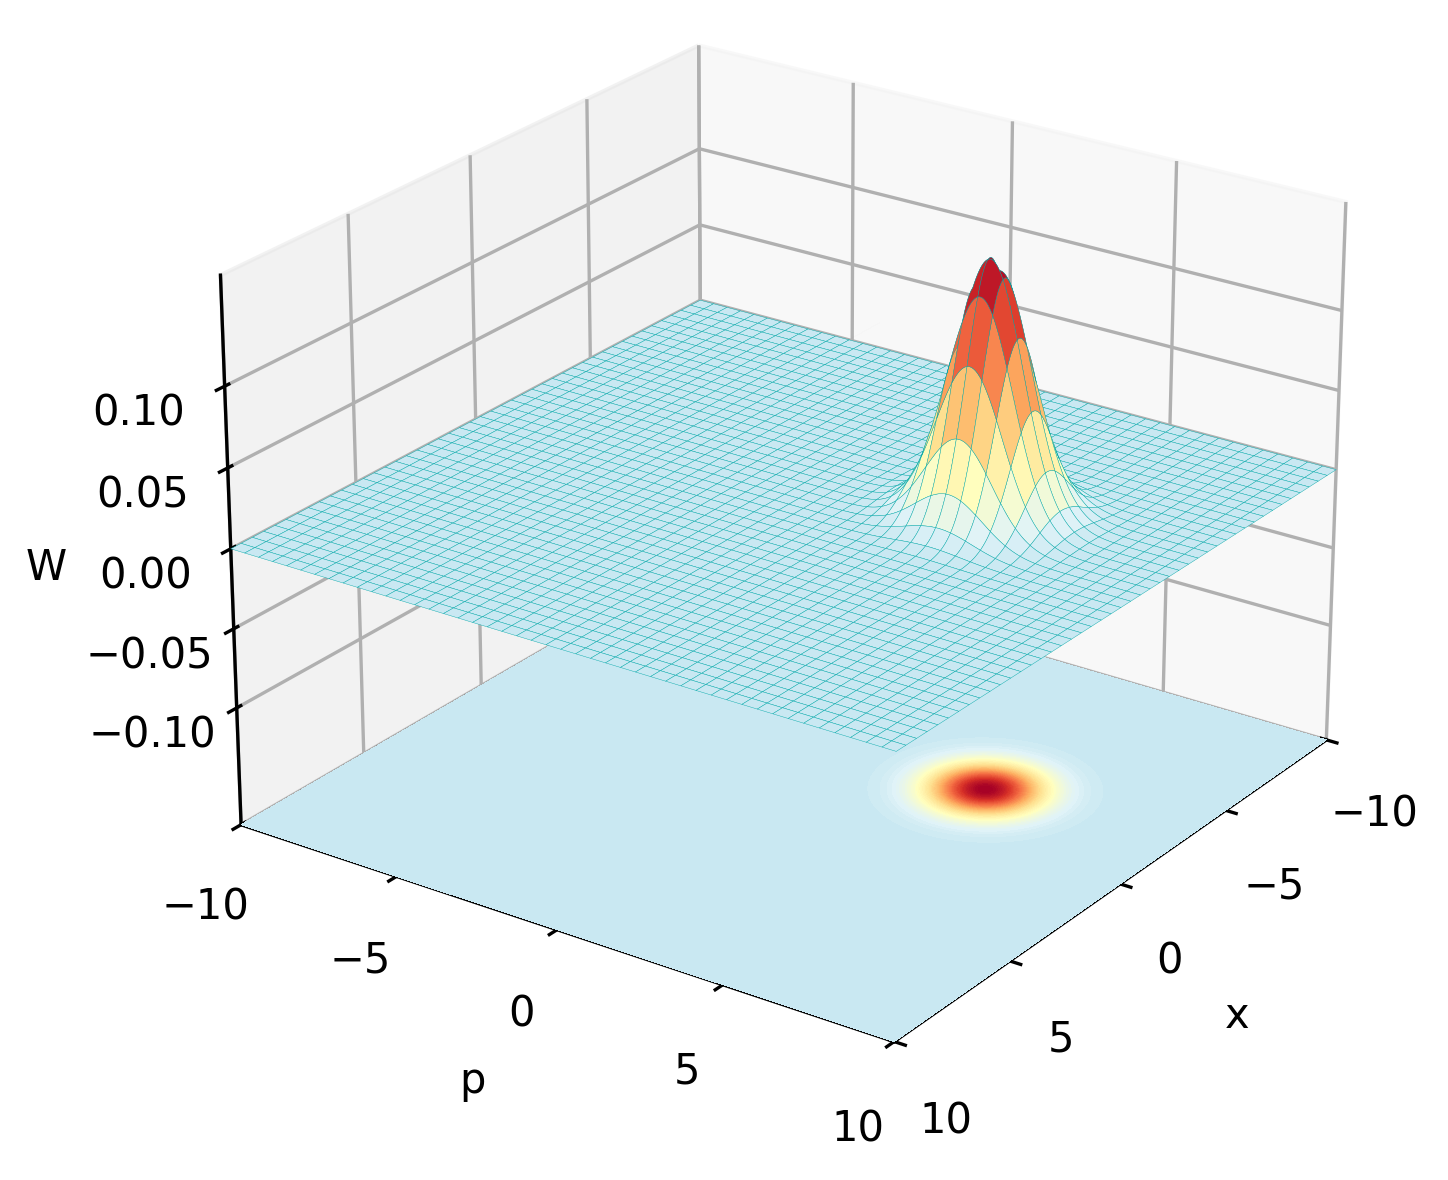
\includegraphics[width=0.45\textwidth, keepaspectratio]{figs/apr_rotacao.png}\quad
                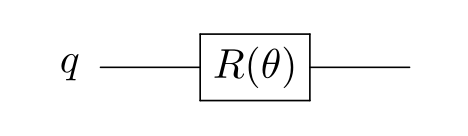
\includegraphics[width=0.45\textwidth, keepaspectratio]{figs/circuito_rotacao.png}\\
                \tiny{Rotação}
            \end{minipage}
            \hfill
            \begin{minipage}[c]{0.45\textwidth}
                \centering
                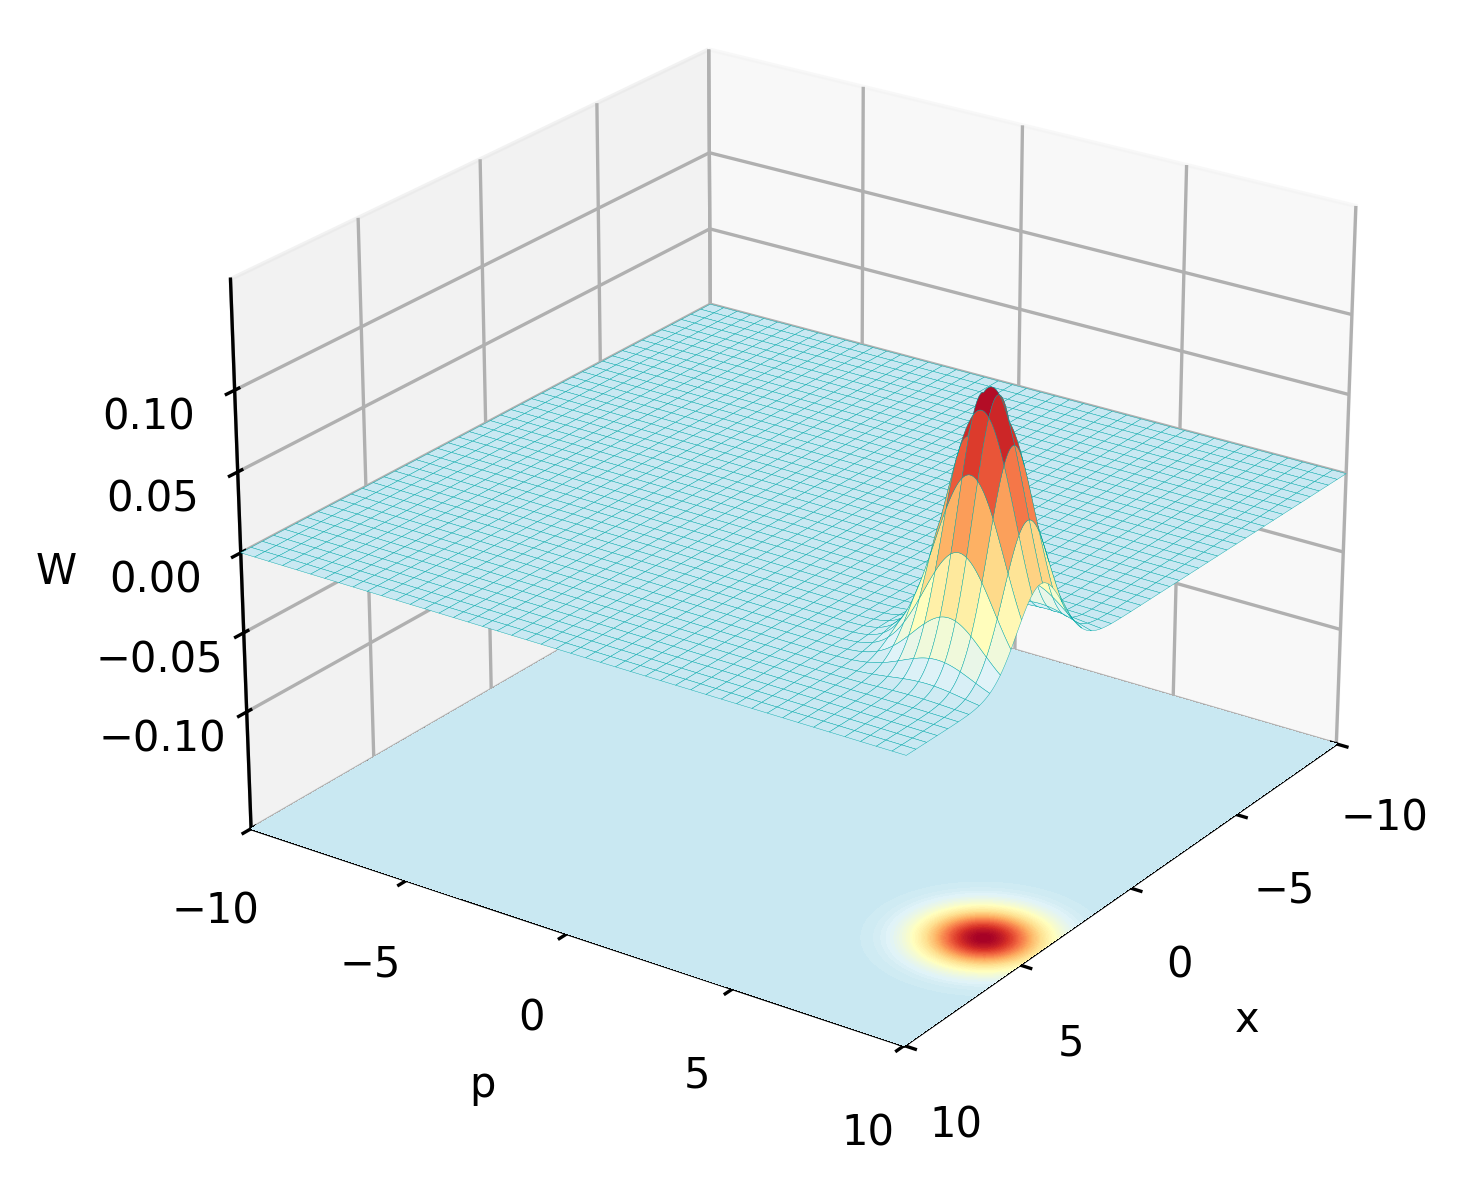
\includegraphics[width=0.45\textwidth, keepaspectratio]{figs/apr_wigner_deslocamento.png}\quad
                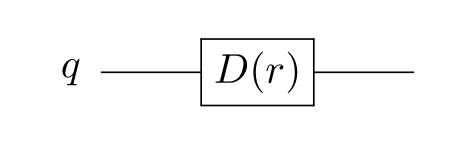
\includegraphics[width=0.45\textwidth, keepaspectratio]{figs/circuito_deslocamento.png}\\
                \tiny{Deslocamento}
            \end{minipage}
        \end{minipage}
        \vfill
        \begin{minipage}[c]{\textwidth}
            \begin{minipage}[c]{0.45\textwidth}
                \centering
                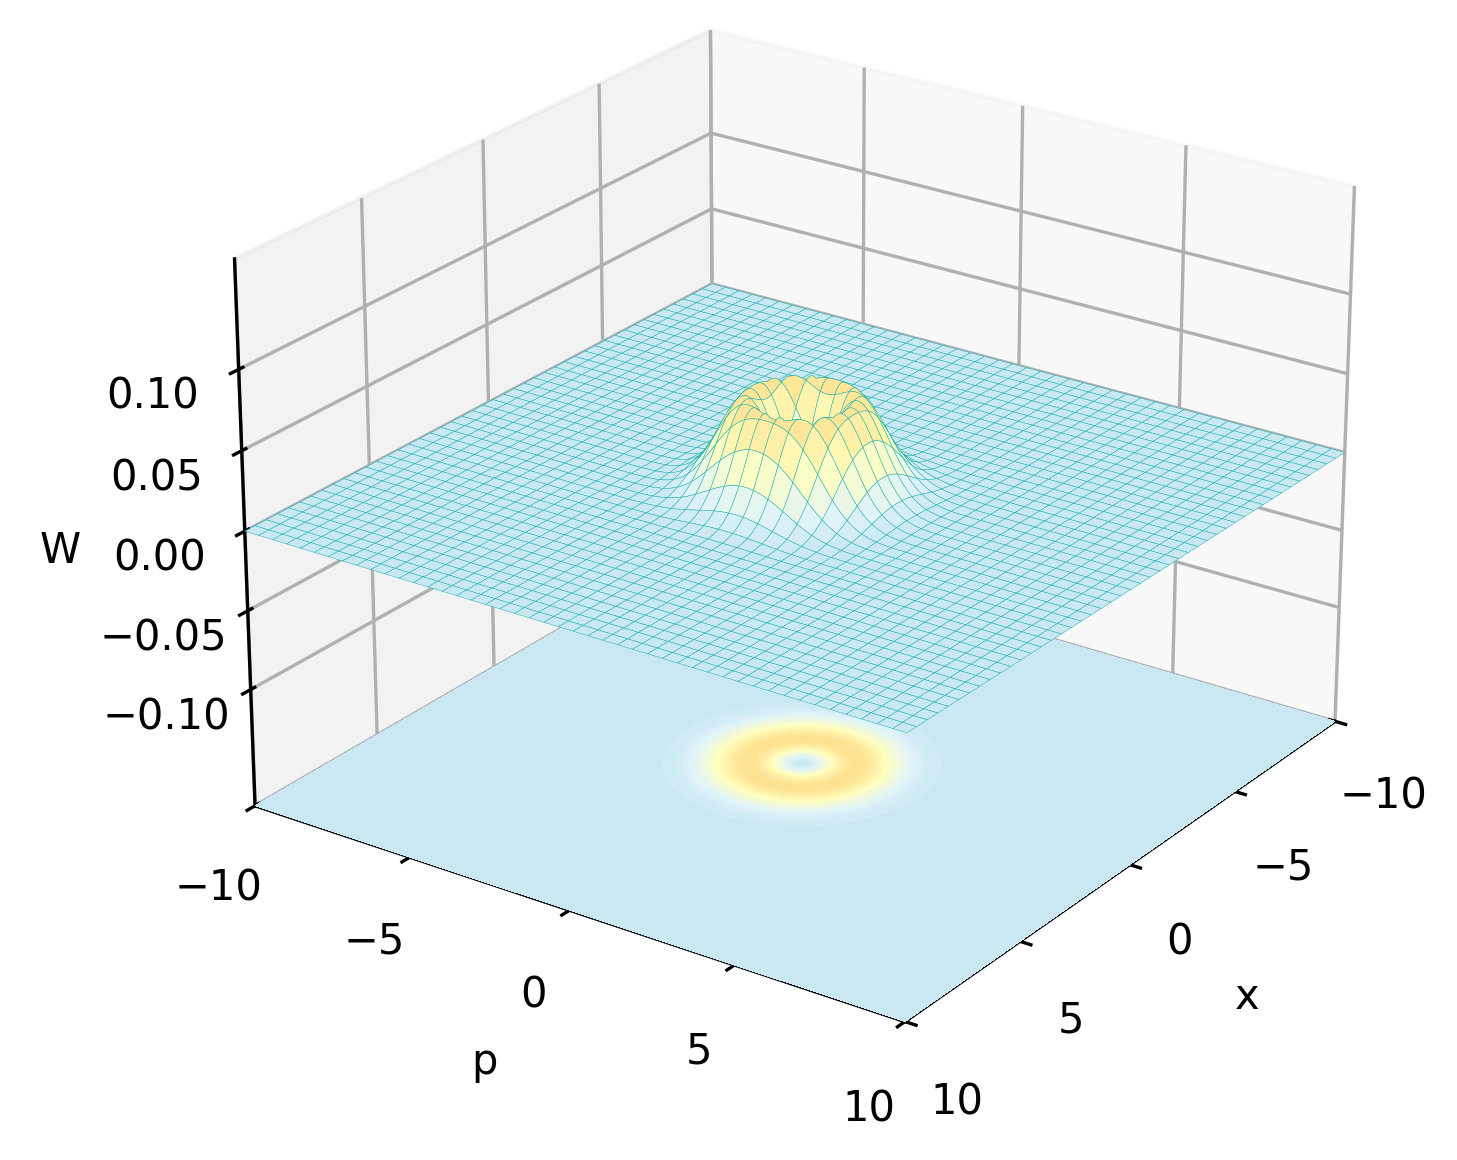
\includegraphics[width=0.45\textwidth, keepaspectratio]{figs/apr_wigner_divisor_de_feixe_fock10.png}\quad
                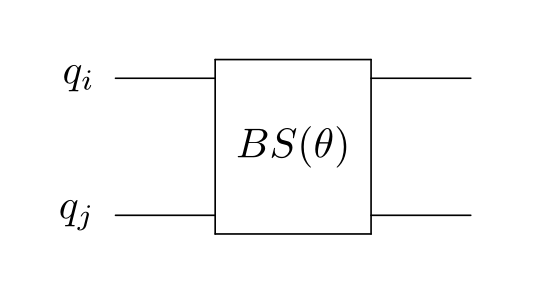
\includegraphics[width=0.45\textwidth, keepaspectratio]{figs/circuito_divisao_feixe.png}\\
                \tiny{Divisão de Feixe}
            \end{minipage}
            \hfill
            \begin{minipage}[c]{0.45\textwidth}
                \centering
                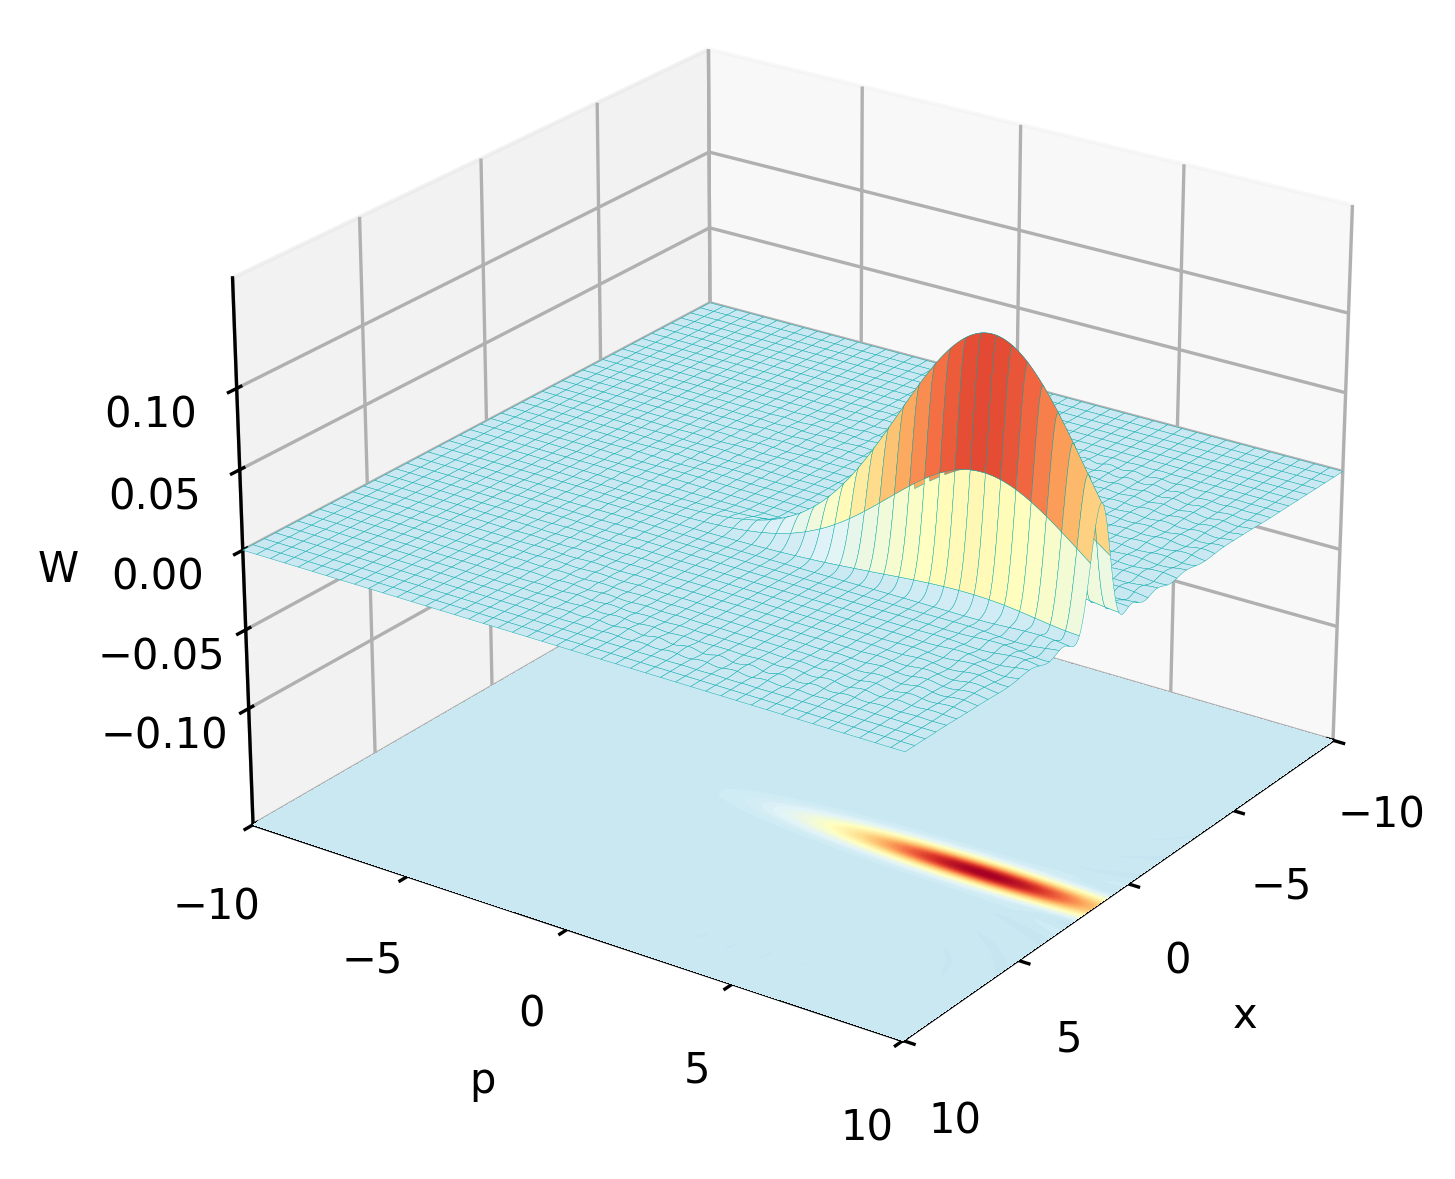
\includegraphics[width=0.45\textwidth, keepaspectratio]{figs/apr_wigner_compressao.png}\quad
                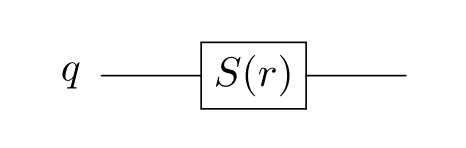
\includegraphics[width=0.45\textwidth, keepaspectratio]{figs/circuito_compressao.png}\\
                \tiny{Compressão}
            \end{minipage}
        \end{minipage}
        \begin{center}
            \tiny{\textbf{Fonte}: Autoria própria (2026)}
        \end{center}
    \end{block}
\end{frame}

\begin{frame}{Computação Quântica de Variáveis Contínuas}

    \begin{block}{Portas Não Gaussianas}
        
        \begin{minipage}[c]{\textwidth}
            \begin{minipage}[c]{0.45\textwidth}
                \centering
                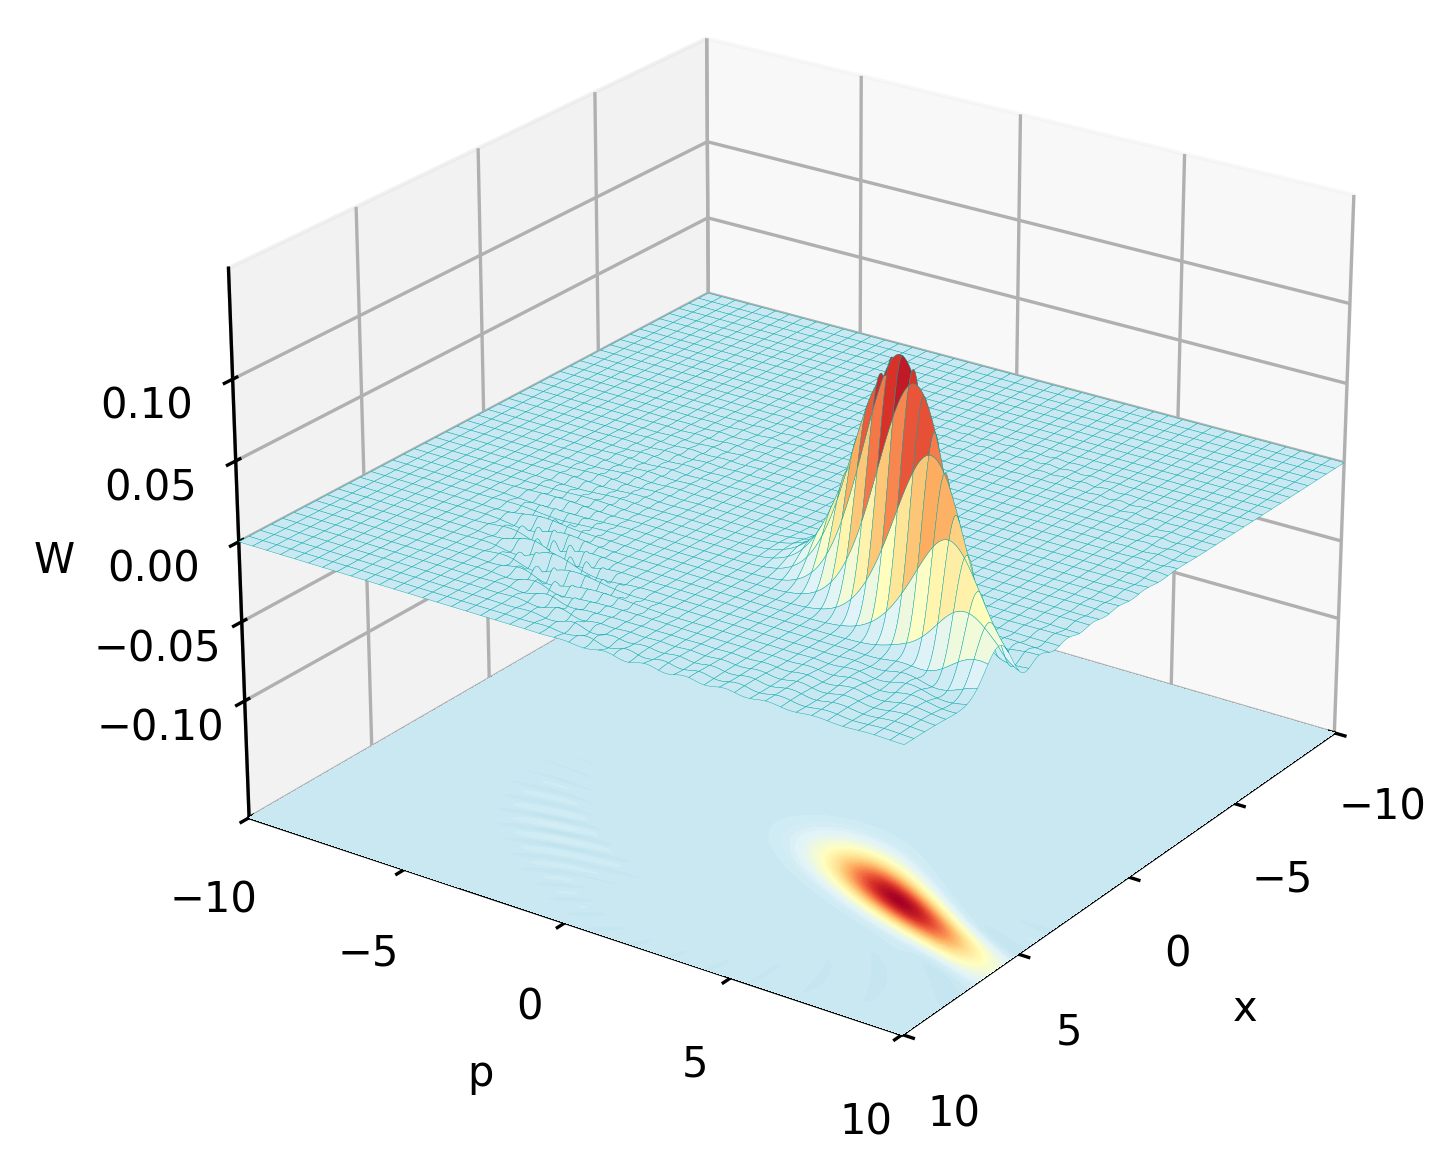
\includegraphics[width=0.45\textwidth, keepaspectratio]{figs/apr_wigner_fase_cubica.png}\quad
                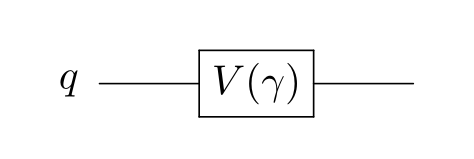
\includegraphics[width=0.45\textwidth, keepaspectratio]{figs/circuito_cubica.png}\\
                \tiny{Fase Cúbica}
            \end{minipage}
            \hfill
            \begin{minipage}[c]{0.45\textwidth}
                \centering
                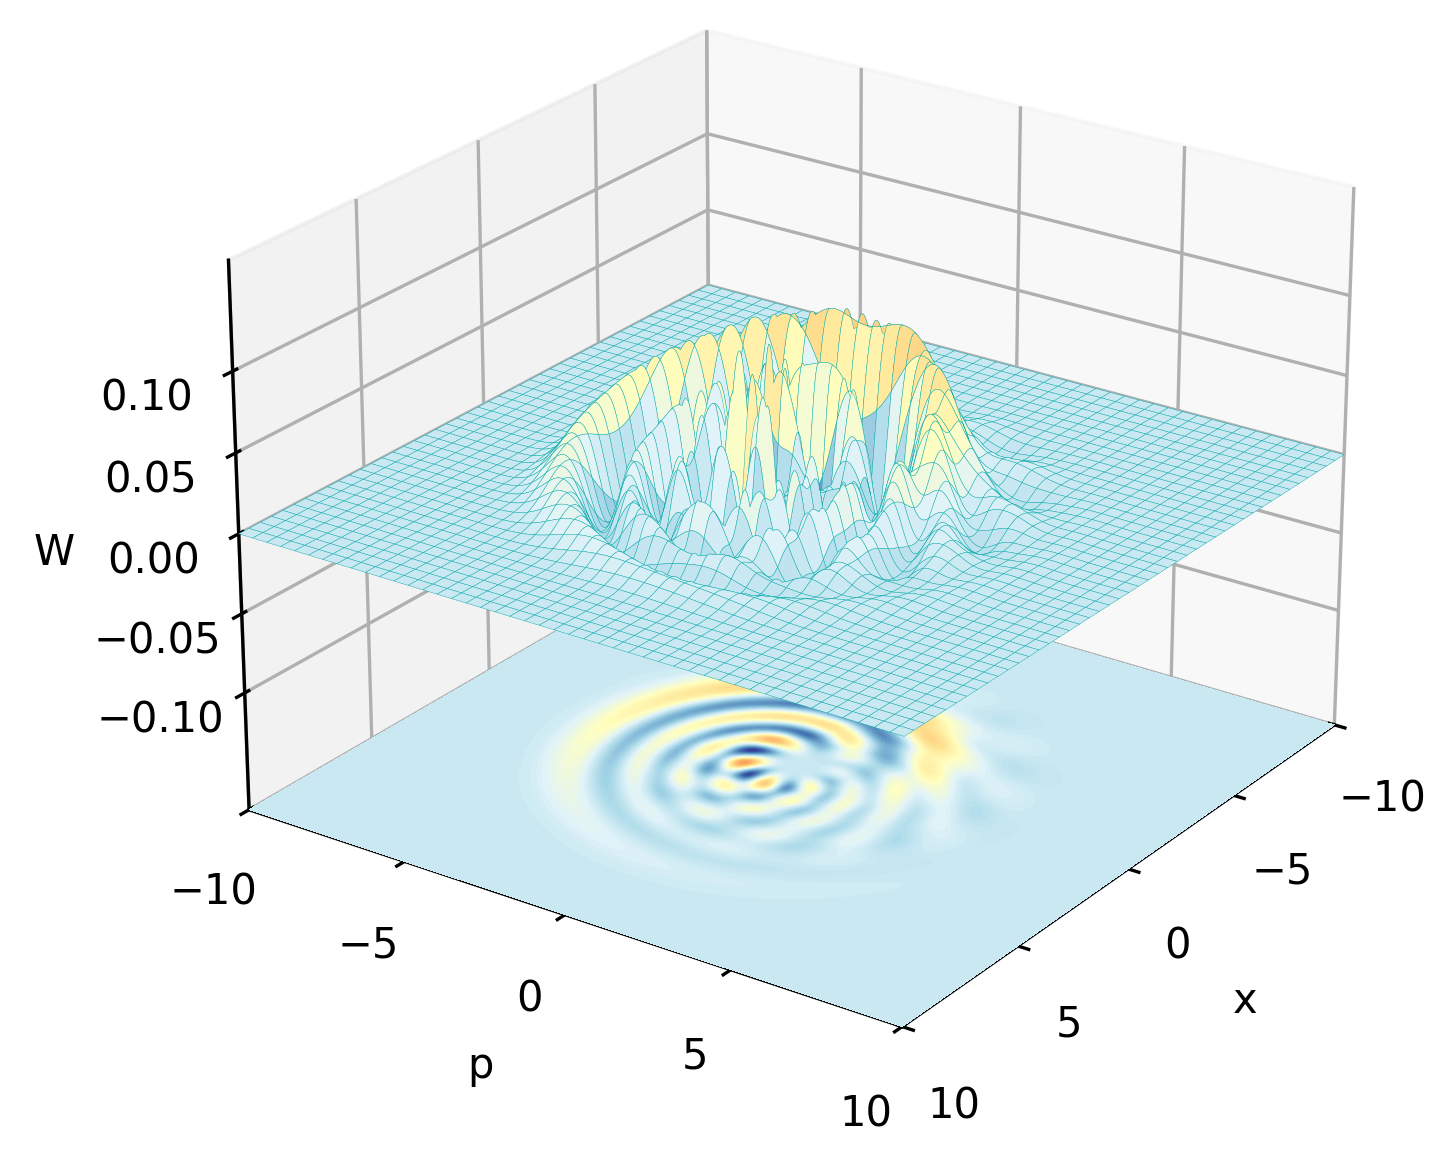
\includegraphics[width=0.45\textwidth, keepaspectratio]{figs/apr_wigner_kerr.png}\quad
                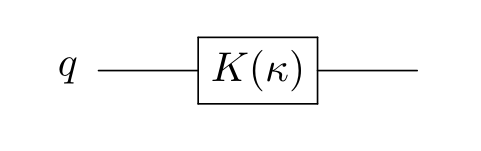
\includegraphics[width=0.45\textwidth, keepaspectratio]{figs/circuito_kerr.png}\\
                \tiny{Kerr}
            \end{minipage}
        \end{minipage}
        \begin{center}
            \tiny{\textbf{Fonte}: Autoria própria (2026)}
        \end{center}
    \end{block}
\end{frame}

%------------------------------------------------
\subsection{Abordagem Quântica}
\begin{frame}{Abordagem Quântica}
    \begin{minipage}[c]{0.45\textwidth}
        
        \begin{block}{Modelo QUBO}
            Função custo para variável binária $x_i\in\{0,1\}$
            $$
            H_{\text{QUBO}} = \sum_{i\in V}a_ix_i + \sum_{i,j\in E}b_{ij}x_ix_j
            $$
        \end{block}
        
        \begin{block}{Modelo Ising}
            Descrição de sistemas físicos $\rightarrow$ spin binário $s_i\in\{-1,+1\}$
            $$
            H_{s} = \sum_{i\in V}h_is_i + \sum_{i,j\in E}J_{ij}s_is_j
            $$
            onde $h_i \rightarrow$ campos locais e\\ $J_{ij}\rightarrow$ acoplamentos entre spins
        \end{block}
    \end{minipage}
    \hfill
    \begin{minipage}[c]{0.45\textwidth}
        \begin{block}{Viabilização da implementação}
            $$x_i=\frac{1+s_i}{2}$$
        \end{block}
    \end{minipage}
\end{frame}


\begin{frame}
    \frametitle{Abordagem Quântica}
    No contexto de CVQC: $x\rightarrow\hat{x}=(\hat{x}_1,\hat{x}_2,\dots,\hat{x}_d)$ 
    Assim a formulação pode ser 
    $$
    \hat{H}=f(\hat{x})+\lambda_h\sum_{r=1}^Rh_r(\hat{x})^2+\lambda_g\sum_{s=1}^S\max\{0,g_s(\hat{x})\}^2+\lambda_b\sum B(\hat{x})
    $$
\end{frame}

\begin{frame}{Abordagem Quântica}

    \begin{block}{Variational Quantum Eigensolver}
        Algoritmo híbrido $\rightarrow$ clássico-quântico 
        $$
            \ket{\psi(\beta)}=U(\beta)\ket{0}^{\otimes n}
        $$

        $$
            \min_{\beta^*} E(\beta^*) =\min_{\beta^*}\bra{\psi(\beta^*)}H\ket{\psi(\beta^*)}
        $$

    \end{block}

\end{frame}

\begin{frame}{Abordagem Quântica}

    \begin{block}{Quantum Approximate Optimization Algorithm}
        Encontrar $(\gamma^*,\beta^*)$ que minimiza
        $$
            F_p(\gamma,\beta)=\bra{\gamma,\beta}H_C\ket{\gamma,\beta}
        $$
        onde o estado parametrizado
        $$
            \ket{\gamma,\beta}=\prod_{l=1}^p e^{-i\beta_lH_M}e^{-i\gamma_lH_C}\ket{\psi_0}
        $$
    \end{block}
\end{frame}
%------------------------------------------------
\section{Objetivos}
\begin{frame}{Objetivos}
    \begin{block}{Geral}
        Desenvolver um modelo baseado em algoritmos de computação quântica de variáveis contínuas para a resolução de problemas de otimização combinatória, com ênfase em instâncias do VRP.
    
    \end{block}

    \begin{block}{Específico}
        \begin{itemize}
            
            \item Investigar modelos fundamentais aplicados ao TSP, com o intuito de avaliar o desempenho e a eficiência das abordagens propostas em um cenário controlado.
            
            \item Propor uma formulação matemática para problemas do tipo VRP que permita sua representação em termos compatíveis com a computação quântica de variáveis contínuas.
            
            \item Estabelecer um mapeamento dessas formulações em Hamiltonianos, viabilizando sua implementação em dispositivos quânticos de variáveis contínuas.
        \end{itemize}

    \end{block}

\end{frame}
%------------------------------------------------
\section{Metodologia e Resultados Parciais}
\begin{frame}{Metodologia e Resultados}
    \begin{block}{Modelagem}
        \begin{itemize}
            \item Duas propostas
            \item Grafo e variáveis
            \begin{itemize}
                \item $N$ cidades
                \item $d_{ij}$ distâncias entre as cidades $i$ e $j$
                \item variável binária
                $$x_{ik}=\begin{cases}
                    1, &\text{se a cidade }i\text{ é visitada na posição }k,\\
                    0, &\text{caso contrário}
                \end{cases}$$
            \end{itemize}
        \end{itemize}
    \end{block}
\end{frame}

\begin{frame}
    \frametitle{Metodologia e Resultados Parciais}

    \begin{block}{Função Objetivo e restrições - TSP}
        $$H=\sum_{k=1}^{N}\sum_{i=1}^{N}\sum_{j=1}^{N} d_{ij}x_{i,k}x_{j,k+1}$$
    sujeito a 
        \begin{itemize}
            \item $\displaystyle\sum_{i=1}^{N} = 1,\ \forall k\in K\rightarrow$ exatamente uma cidade, 
            \item $\displaystyle\sum_{k=1}^{N} = 1,\ \forall k\in K\rightarrow$ cada cidade deve ser visitada uma única vez
        \end{itemize}
    \end{block}

\end{frame}

\begin{frame}
    \frametitle{Metodologia e Resultados Parciais}
    \begin{block}{Algoritmo de Força Bruta}
        \begin{itemize}
            \item Base comparativa
            \item quantidade de variáveis binárias pequenas
            \item possibilidade de obter todas as rotas possíveis
        \end{itemize}
    \end{block}
    \pause 
    \begin{block}{Ambiente Computacional}
        Chamado Beluga, equipado com:
        \begin{itemize}
            \item processador AMD EPYC 7453,
            \item 1TB RAM 
            \item duas GPUs
            \item QuTiP
        \end{itemize}
    \end{block}
    

\end{frame}

\begin{frame}
    \frametitle{Metodologia e Resultados Parciais}

    \begin{block}{Modelagem qubits$\rightarrow$qumodes}
        \begin{itemize}
            \item variáveis discretas $x_{ik}\rightarrow x'_{ik}\rightarrow \hat{x}_{ik}=\displaystyle\frac{1+x'_{ik}}{2} \rightarrow\hat{x}_{ik}$ operador de posição e $\hat{p}_{ik}$ operador de momento 
            \item $[\hat{x}_{ik},{\hat{p}_{kl}}]=i\hbar\delta_{ij}\delta_{kl}$
            \item poço duplo $H_{\text{bin}}=\displaystyle\sum_{i,k}\left(\left(x'_{ik}\right)^2-1\right)^2$
            \item termo cinético $\displaystyle\sum_{i,k}\frac{\hat{p}^2_{ik}}{2m}$
        \end{itemize}
    \end{block}

\end{frame}

\begin{frame}
    \frametitle{Metodologia e Resultados Parciais}

    \begin{block}{Hamiltoniano completo}
        \begin{equation*}
            \begin{split}
                H=&   \sum_{k=1}^{N}\sum_{i=1}^{N}\sum_{j=1}^{N} d_{ij}x_{i,k}x_{j,k+1} + \\ 
                & + \alpha\sum_{i=1}^{N}\left(\sum_{k=1}\hat{x}_{i,k}-1\right)^2 +
                \beta\sum_{k=1}^{N}\left(\sum_{i=1}\hat{x}_{i,k}-1\right)^2 +\\
                & + \gamma\sum_{ik}\left(\left(x_{ik}\right)^2-1\right)^2 
                 + \sum_{ik}\frac{\hat{p}^2_{ik}}{2m}
            \end{split}
        \end{equation*}
        onde $\alpha, \beta,\gamma$ e $m$ são hiperparâmetros do modelo
    \end{block}

\end{frame}

\begin{frame}{Metodologia e Resultados Parciais}
    \begin{block}{Resultados}
        \begin{itemize}
            \item $n\in\{3,4\}\rightarrow$ 
            \begin{itemize}
                \item Comparação com resultados de força bruta
                \item Equivalente 
                
                Exemplo: 
                \begin{itemize}
                    \item Força Bruta: $V_0\rightarrow V_1\rightarrow V_2\rightarrow V_3\rightarrow V_0$
                    \item Método Qubit-Qumode: $V_0\rightarrow V_3\rightarrow V_2\rightarrow V_1\rightarrow V_0$
                \end{itemize}
            \end{itemize}
        \end{itemize}
    \end{block}
\end{frame}

\begin{frame}{Metodologia e Resultados Parciais}
    \begin{block}{Resultados}
        \begin{itemize}
            \item Intâncias de pequena dimensão
            \item custo de memória: $O(2^M)$ qubits $\rightarrow O(d^M)$ qumodes
        \end{itemize}
    \end{block}
\end{frame}

\begin{frame}{Metodologia e Resultados Parciais}
    \begin{block}{Modelo $N-$qumode-posição}
        \begin{itemize}
            \item Cada posição da rota uma variável indica qual cidade é visitada 
            \item Exemplo 
            \begin{itemize}
                \item para $N=4\rightarrow \ket{2\ 0\ 3 \ 1}$
            \end{itemize}
            \item Nesse contexto: 
            \begin{itemize}
                \item cidade $c_k\in\{0,1,\dots,N-1\}$
            \end{itemize}
        \end{itemize}
    \end{block}
\end{frame}

\begin{frame}{Metodologia e Resultados Parciais}
    \begin{block}{Hamiltoniano}
        \begin{itemize}
            \item Custo $H=\sum_{k=1}^{N} d_{n_k,n_{k+1}}$ 
            \item Operador numero $\hat{n}_k\ket{a}=a\ket{a}$
            \item Hamiltoniano correspondente
            $$
            H=\sum_{k=1}^{N} \sum_{a=1}^{N}\sum_{b=1}^{N} \ket{a}\bra{a}_k\otimes\ket{b}\bra{b}_{k+1}
            $$
        \end{itemize}
    \end{block}
\end{frame}

\begin{frame}{Metodologia e Resultados Parciais}
    \begin{block}{Penalidades}
        \begin{itemize}
            \item Apenas uma cidade na rota $$H_{\text{penalty}}=\sum_{k<l} \ket{a}\bra{a}_k\otimes \ket{a}\bra{a}_l$$
        \end{itemize}
    \end{block}
\end{frame}

\begin{frame}{Metodologia e Resultados Parciais}
\begin{block}{Hamiltoniano}
    $$H=\sum_{k=1}^{N} \sum_{a=1}^{N}\sum_{b=1}^{N} \ket{a}\bra{a}_k\otimes\ket{b}\bra{b}_{k+1} +\lambda \sum_{a=1}^{N}\left(\sum_{k<l} \ket{a}\bra{a}_k\otimes \ket{a}\bra{a}_l -1\right)^2$$

    onde $\lambda$ é um parâmetro de penalização
\end{block}
\end{frame}

\begin{frame}{Metodologia e Resultados Parciais}
    \begin{block}{Comparação de Resultados}
        \centering
        \begin{tabular}{|c|c|c|r|}
    \hline
    \textbf{N} & \textbf{Custo} & \textbf{Energia} & \multicolumn{1}{c|}{\textbf{Tempo}} \\ \hline
    3 & 19 & 19,0 & 6 ms \\ \hline
    4 & 23 & 23,0 & 16 ms \\ \hline
    5 & 12 & 12,0 & 86 ms \\ \hline
    6 & 19 & 19,0 & 1 s 229 ms \\ \hline
    7 & 41 & 41,0 & 1 min 7 s \\ \hline
    8 & 26 & 26,0 & 2 h 53 min \\ 
    \hline
    9 & 17 & 17,0 & 3sems 20h 1min 35s\\ \hline
    \end{tabular}\\ 
    \tiny{Autoria própria (2026)}
    \end{block}
\end{frame}

\begin{frame}{Metodologia e Resultados Parciais}

    \begin{block}{Comparação Estrutural}
        \centering
        \begin{tabular}{lcc}
        \hline
        \textbf{Característica} & \textbf{Proposta 1} & 
        \textbf{Proposta 2} \\
        \hline
        Variáveis & $N^2$ binárias & $N$ qumodes \\
        Corte local & --- & $d = N$ \\
        Dimensão do espaço & $2^{N^2}$ & $N^N$ \\
        Exemplo $N=6$ & $2^{36} \approx 6{,}9 \times 10^{10}$ & 
        $6^6 = 46.656$ \\
        Exemplo $N=8$ & $2^{64} \approx 1{,}8 \times 10^{19}$ & 
        $8^8 = 16.777.216$ \\
        % Restrições & Termos de penalização & Termos de penalização \\
        % Hardware natural & Qubits & Fotônico/CV \\
        \hline
        \end{tabular} \\
        \tiny{Autoria Própria (2026)}
    \end{block}
\end{frame}

%------------------------------------------------
\section{Conclusões e Próximo Passos}
\begin{frame}{Conclusão e Próximo Passos}
    \begin{block}{Conclusão}
        \begin{itemize}
            \item Desenvolvimento de abordagem em CVQC para TSP/VRP 
            \item Duas formulações 
            \item Resultados obtidos demonstram a consistência da formulção 
        \end{itemize}
        
    \end{block}
\end{frame}

\begin{frame}{Conclusão e Próximo Passos}
    \begin{block}{Próximos Passos}
        \begin{itemize}    
            \item Aplicar modelos de otimização $VQE$ ou $QAOA$
            \item Modificar o Hamiltoniano para um VRP 
            \begin{itemize}
                \item Proposta inicial
            \end{itemize}
        \end{itemize}

        \begin{equation*}
            H^{(M)}_{cost} =  \sum_{\mu=1}^{M} \sum_{a=1}^{N-1} \sum_{i=1}^{N} 
            \sum_{j=1}^{N} d_{ij} \left(\ketbra{a}{a}^{(n)}_k \otimes 
            \ketbra{\mu}{\mu}^{(v)}_k\right)  \left(\ketbra{a}{a}^{(n)}_j \otimes \ketbra{\mu}{\mu}^{(v)}_j\right)    
        \end{equation*}
        
    \end{block}
\end{frame}

\begin{frame}{Conclusão e Próximo Passos}
    \begin{block}{Próximos Passos}
        \centering
\resizebox{\textwidth}{!}{
    \begin{tabular}{|p{6.2cm}|c|c|c|c|c|c|c|c|c|c|c|c|c|}
    \hline

    \textbf{Etapa} & \textbf{Jun} & \textbf{Jul} & \textbf{Ago} & \textbf{Set} & \textbf{Out} & \textbf{Nov} & \textbf{Dez} \\  \hline \hline
    Revisão bibliográfica e ampliação do referencial teórico &  \cellcolor{gray}  &  \cellcolor{gray}  &  \cellcolor{gray}  &     &     &     & \\  \hline
    Desenvolvimento e extensão do Hamiltoniano               &  \cellcolor{lightgray}  &  \cellcolor{lightgray}  &  \cellcolor{lightgray}  &  \cellcolor{lightgray}  &     &     & \\  \hline
    Implementação computacional  & &  \cellcolor{gray}  &  \cellcolor{gray}  &  \cellcolor{gray}  &  \cellcolor{gray}  &         & \\  \hline
    Simulações, análise de resultados e validação            &     &     &  \cellcolor{lightgray}  &  \cellcolor{lightgray}  &  \cellcolor{lightgray}  &     & \\  \hline
    Redação e consolidação da tese &  \cellcolor{gray}  &  \cellcolor{gray}  &  \cellcolor{gray}  &  \cellcolor{gray}  &  \cellcolor{gray}  &  \cellcolor{gray}  & \\  \hline
    Defesa da Tese &    &    &    &     &     &      & \cellcolor{lightgray}  \\  \hline
    \end{tabular}
    }
    \tiny{Autoria Própria (2026)}

    \end{block}
\end{frame}

%------------------------------------------------
\begin{frame}
    \titlepage
\end{frame}

\end{document}